% --- Preamble Contents --- %
\documentclass[12pt,a4paper,twoside]{report}

\def\mydate{\leavevmode\hbox{\twodigits\day/\twodigits\month/\the\year}}
\def\twodigits#1{\ifnum#1<10 0\fi\the#1}
\setcounter{tocdepth}{4}
\setcounter{secnumdepth}{4}
\usepackage{hyperref}
\usepackage{graphicx}
\usepackage[margin=1.0in]{geometry}
\usepackage[english]{babel}
\usepackage[T1]{fontenc}
\usepackage[utf8]{inputenc}
\usepackage{siunitx}
\usepackage{amsmath}
\usepackage{amsfonts}
\usepackage{amssymb}
\usepackage{caption}
\usepackage{color}
\usepackage{placeins}
\usepackage{listings}
\usepackage{float}
\renewcommand\thesection{\arabic{section}}
\captionsetup{labelfont=bf}
\captionsetup{justification=centering}
\usepackage[superscript,biblabel]{cite}
\usepackage{cancel}
\makeatletter \renewcommand{\@citess}[1]{\textsuperscript{\,[#1]}}
\usepackage[table,xcdraw]{xcolor}

\usepackage{slashbox}
\usepackage{fontspec}
\setmainfont{Arial}
\usepackage{multirow}
\usepackage{pdfpages}





% --- Document Start --- %
\begin{document}
% --- Title Construction ---%

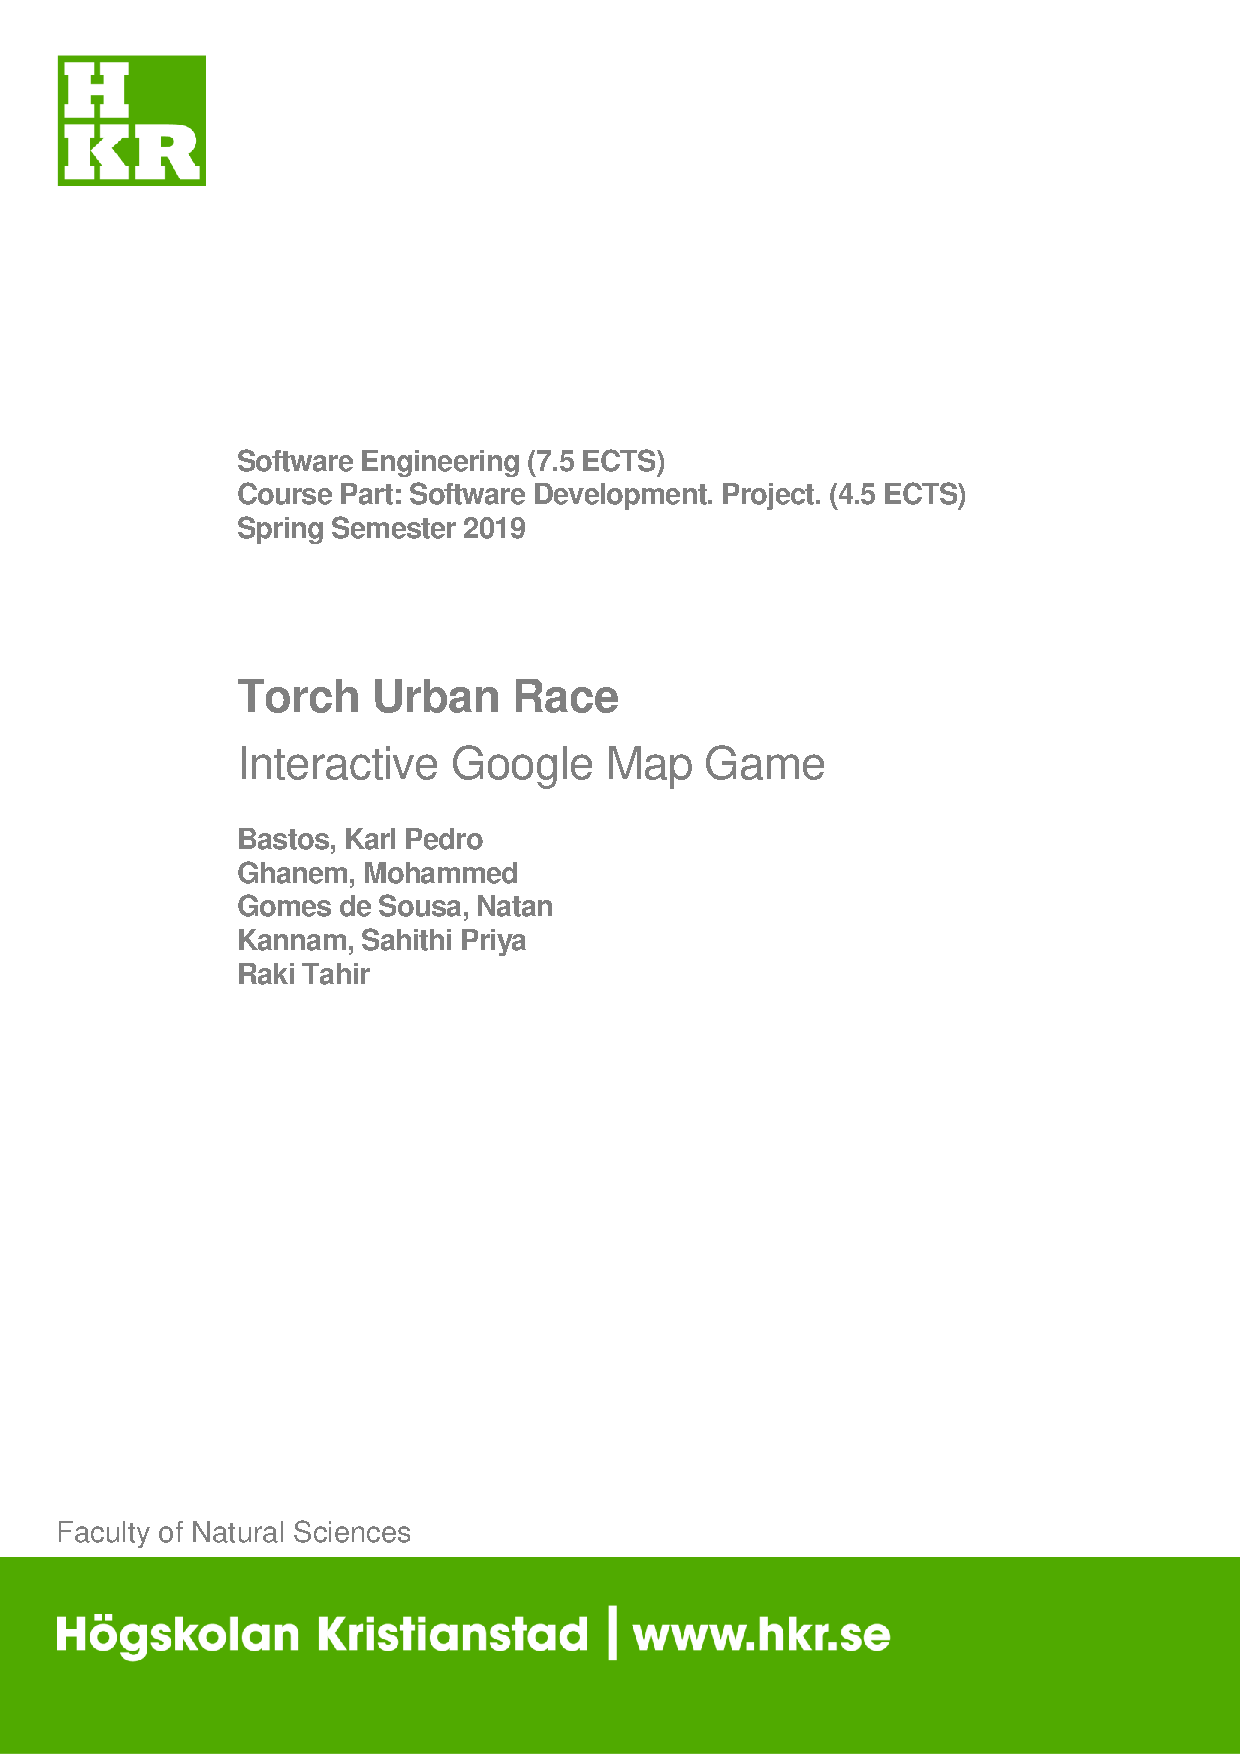
\includepdf[pages=-]{handsomebunny.pdf}
%The title page, any modification should be done on the initial docx file and reupload the pdf file into latex 


% --- Title Construction ---%
\newpage
\noindent \textbf{Author} \\
 Bastos, Karl Pedro \\
 Ghanem, Mohammed \\
 Gomes de Sousa, Natan \\
 Kannam, Sahithi Priya \\
 Raki, Tahir  \\
 
\noindent \textbf{Title}\\
Torch Urban Race\\

\noindent \textbf{Supervisor}\\
Marijana Teljega, Nils Svensson\\

\noindent \textbf{Course Examiner}\\
Daniel Einarson\\

\noindent \textbf{Abstract }\\
This report presents a Google Maps based Android game. The purpose is to go around the map in real life to pickup and travel with these torches. This idea was inspired by the Olympic torch relay and acts as a fun motivator to move more. The purpose of this report is to examine performance between two different architectures. The first architecture has all calculations and number crunching on the server side. The second architecture, has all the number crunching on the client side. 

The results of this research show response time increasing drastically with respect to three factors: number of torches in the system, number of clients being serviced and network access type. However, the client side architecture was unaffected by these factors with the only variable being processing power.

\noindent \textbf{Keyword }\\
Android, Game, GPS, Google Maps, Server, Client, XP

\newpage
\tableofcontents
\newpage 
%%%%%%%%%%%%%%%%%%%%%%%%%%%%%%%%%%%%% Start

\section{Introduction}
In July 2016, Pokémon Go was published and achieved a huge impact on the world of mobile phone games\cite{2}. The basic concept of this game is to control the movement of your character by moving the position of your phone to find and catch Pokémon which virtually spawn at real locations, but can only be seen through the app. Taking this as inspiration, the idea to this project arose: to produce a game-like app which uses the phone's position for the character movement and the Olympic games as a theme. As Vidar Eilertsen said, “The flame is a symbol of the Olympic message of peace, friendship, tolerance and hope”\cite{18}. The Olympic games held once in every four years, starts with the Olympic relay which transports the flame from Greece to the country hosting the Olympic games. To participate physically and be part of this flame relay of friendship, tolerance, and hope is difficult. Torch - Urban Race will make it simple and bring this significant historic event right to users’ phones, which allows users to feel the history, build friendships and exercise while playing the game and enjoying the beauty of areas around them\cite{10}\cite{16} .

The app will feature an Olympic torch which will be started at a certain location and can be carried by the user to different locations to achieve a run around the world. Anyone with the app will be able to see the current location of the torch, pick it up and carry it to a different location. Also, there will be smaller, custom torches that can be privately shared with friends or public ones by companies, e.g. for advertisement. People will be motivated through this app to follow the progress of the Olympic torch and go out with their own personal torches to compete with friends.

With mobile games becoming more popular and almost everyone owning a phone capable of running games it is becoming increasingly important to create severs that can handle large amounts of players. Video games are the worlds most popular form of entertainment stated by Angelo M. D'Argenio. In 2018, 48\% of revenue made by the video game industry was in mobile games. Some of the most popular games in the world such as League of Legends and Fortnite are multiplayer games. This means it becomes more important to make sure that developers make severs that can handle a large player base. The Torch app will be tested to see what is better for mobile games. Either, if it is more efficient to keep most of the core game functions on the sever side or to make the client do most of the work. The results will help developers to make the correct choice for their products\cite{15}.
\newpage
\subsection{Background}

Multiplayer games have always been difficult to handle compared to other forms of internet connections. With websites one just requests the data from the sever. Even video calls are easier to construct since the simplex conversation between the people means that most people won't recognize a delay or small loss of data between the callers. When it comes to games speed and data-loss becomes a much more important issue. Speed of requests become a very important factor especially in real time game. Not only do the players need to have a fast response time but also a stable connection. To illustrate, here is a simple example about two players playing catch with a ball. If a player throws the ball the information has to be sent to the sever and then from sever to the other player. If this processes is too slow the catching player won't receive the notification until it is too late and the ball already passed. Likewise if the player catching the ball sends the catch command too slow the ball will just fly by the catching player. If one player constantly disappears from the caching game due to signal drop this will also frustrate both players and make a game impossible. This applies to all games, even turn-based games, although those have a much more lax setting on time constraints. But when it is the players turn, the command should have an impact as soon as possible and not take several seconds to execute. As you can tell games have a very strict time constraints to make them fun.

Severs become even more important as the multiplayer games involve more players. The more players, the higher the request. Thus creating the most efficient system is not only important for the players, but as well as for the developers making the correct choice when designing the program structure. Since it will be much more expensive revamping the system once it made, building a correct base the first time is priority. 

What we will be testing is to see how the architecture of sever should be made. In particular, should the working load be heavier on the client (player side) or server. This question becomes more tricky when dealing with mobile phones. Since mobile phone generally have much less resources than the host running the server such as smaller GPU and CPU. One example might be mobile devices generally have passive heat sinks instead active ones such as fans on the CPU. This means a local sever host has allot more options to upgrade and improve its resources. Running on a faster machine would make a game run faster for the mobile phone. Since mobile online multiplayer gaming is a quite recent there aren't many resources online in creating the sever for your mobile game compare to the other gaming platforms. This is what this project will try to cover. 

By testing out own app, the TorchUR we are trying to see what kind of sever setup would function best for a multiplayer game based on a GPS system like Pokémon GO.

\newpage
\subsection{Aim and Purpose}
\subsubsection{Research Question}
Is it more effective to have the client handle the information and use the server to store and share the data with a database or is it more effective to have the server being responsible for the calculations and processing while the client will only handle the displaying of information?
\subsubsection{Scope and Limitations}
As the size of our team is small and the time-frame of this project is tight, we have several limitations in our methodology. The first limitation is scale. As we do not have an actual server machine to run our back-end on we will be using a regular desktop computer. Additionally, we can't stress test the system with more than 10 clients as we do not have that many phones or friends to help us out (sad).

The second problem is consistency, the Android platform is used by several smartphone manufacturers which all have different hardware specifications. This means that tests on the client side can be vastly different as the smartphone could be more or less powerful.

Another limitation is that of resources, to measure performance we do not have specialized tools, therefore we can only use delta time measurements as an indicator of responsiveness as a metric.

The last limitation is the network stability. This one is dependant on mediators which we cannot account for. Our client relies on their connection to the server to update data. Should that connection be unstable a lot of time could be lost waiting for a response. These limitations combined tell us that the data we can extract and metrics we use to measure performance are not indicative of real-world results, but rather we can only measure relative performance between server side and client side operation.
\newpage
\section{Method}

\subsection{Literature Review}
Since game servers are the essential central piece it is very important to make sure the server is set up as optimally as possible to avoid results such as the Pokémon Go’s initial release that wasn't prepared for the amount of players they were going to have\cite{13}. This caused many players to go without the product of Pokémon Go for several weeks or even months. So finding out the most efficient server setup for a game in the scale of Pokémon Go will be an important information for all future projects that aim for such heights.

We took articles that covered models for server-client applications\cite{12}. This is a very important topic for online multiplayer games since the most popular games tend to be multiplayer games featuring hundreds of players with very good servers. Besides Pokémon Go, there aren't many games that feature a similar GPD based concept. Since Pokémon Go haven’t released any articles on the server we will have to make use of other sever articles that we will adjust to our case.

The articles which were considered where chosen according to how accurately they dealt with the questions. Thanks to Google, very fitting articles could be found easily and only few articles considered were discarded. They all included some helpful information and gave a diverse answer to each question.

This article is about creating and analyzing severs for mobile multiplayer games\cite{14}. Handling severs for phone games is more difficult due to hardware limitations and unstable connections. For this reason the author uses a turn-based game instead which requires less response time and speed then a real time game would such as a first-person shooter and real-time strategy game. The severs are analyzed based on their CPU, RAM and band-width consumption. While the bandwidth was not tested in this report, the sever was used to solve the C10k. C10k is the problem of optimizing the sever to handle many users, as well as a general stress test. This was trying to get 50,000 connections to connect to the sever while the sever only accepted a maximum of 16,000 connections. During the test it handled the 16,000 connections flawlessly, but consumed 3GB of RAM and did not throttle the 2.6 GHz core. Since the author did not have anything to compare this result to any other studies or reference data it actually does not really mean anything. Although the bandwidth was untested, the author claims that it should use less bandwidth due to using an application layer protocol design, compared to using the HTTP. It is unclear how the author came to this conclusion. While it was stated that his limitation is that the sever is not running a full game yet, which would take an increase of all hardware to be able to handle 16,000 connections. The article concludes that creating a self-made sever for a mobile game is completely feasible and it is not necessary because one can also rely on a larger cooperation service so that one could enter in the market with a small budget.

The main conclusion is that the best way to set up a server depends on the number of clients and how much the server needs to compute per request. As such a common theme appeared in many resources is server testing. This means many stress tests are run on the servers to see what is the most effective setup for the game. It seems like having the heavy lifting done by the server provides better performance in general.
\newpage
\subsection{Case Study}
To answer our research question and the finding of the literature review we designed methods for bench testing the responsiveness of the system whether it is on the server side or the client side. Team members and friends were asked to install the application and perform tasks on it. For each task delta time was measured from request to response. The tests were ran in several different configurations. When testing the server side configuration the tests went as follows. Have a client request a distance check on their profile in Km after dropping a torch. The server should calculate based on change in latitude and longitude how much the user has traveled and convert that to Km. This operation was repeated for a single client request then incremented up to 3 clients. In the client side implementation, the distance calculation was done by the client and only the result was sent to the server to be stored in the database. This was tested on 3 different clients as well. The assumption was made that the calculation would not be affected by the server response time if it was running on the client. However, to be sure additional tests were conducted when only 1 client was being serviced incremented by one until a total of 3 clients. The server was monitored to see if some errors occurred. Another test was made to see if the load on the client side and server side affected the response in a less stable network environment. Therefore the test was run using Wi-Fi and mobile 4G network. The results from these experiments will be used as a measurement of effectiveness. The less time it takes to respond to the request the more effective the system is. This is what the team has decided to take into account although it is clearly a limited approach.

\subsection{Working Process}
Through this project, the team focused on adhering to the Extreme Programming ideals. A Trello board was created in order to divide the project into smaller tasks which are easier to manage (Figure \ref{fig:Trello}). Since the iterations are on a week by week basis, we assigned  different priorities to the tasks to make sure that we focused on the most important tasks for the week. A log was setup to make sure that the group is working to the weekly amount exactly twenty hours every week. In addition, to track our progress we also had breakdown charts showing our overall progress and the deadlines. This made it visible to the whole team what was being worked on and by which team member.

The team made extensive use of pair programming. Even without physical presence the group used tools like team-viewer and discord to have the same experience even when not in same place. For the first iteration, the focus was more on getting familiar with Android studio as the team was made up of embedded systems engineers. For the later iterations, the development of the GUI, setting up the database, merging client class with the app and merging server with the database was the focus. 

Throughout the development processes the code was continuously tested. The project used Git as version control software with the repository hosted on GitHub for efficiency and better control of the software (Figure \ref{fig:GitHub}). For every iteration, a story card was made as requested by the client. Then the story card was broken down to task cards, so that each student got to work on their task to fill the ideal 20 hours.

For example, the story card for the second iteration and the respective task cards were as follows

\begin{table}[htps]
\centering
 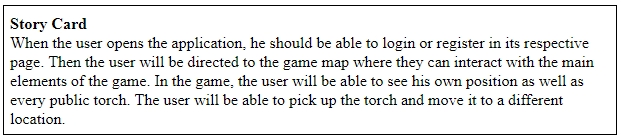
\includegraphics[width=0.9\linewidth]{StoryCard.jpg}
 
\end{table}

\begin{table}[]
    \centering
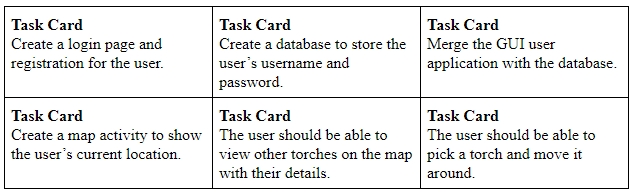
\includegraphics[width=0.9\linewidth]{TaskCard.jpg}
\end{table}

\begin{table}[htps]
\centering
\begin{tabular}{|c|c|c|c|c|c|c|}\hline
\backslashbox{\textbf{Velocity}}{ \ \textbf{Iteration}}
&\makebox[3em]{1}&\makebox[3em]{2}&\makebox[3em]{3}
&\makebox[3em]{4}&\makebox[3em]{5}&\makebox[3em]{6}\\\hline\hline
Student 1 &0.4&0.8&1&0.8&0.8&1\\\hline
Student 2 &0.4&0.4&0.6&1.05&0.65&0.9\\\hline
Student 3 &1.15&1.2&0.9&1.05&1.15&1.2\\\hline
Student 4 &1&0.5&1.05&0.9&1&0.95\\\hline
Student 5 &0.4&0.75&0.8&0.75&0.85&0.6\\\hline
Total velocity &0.67&0.73&0.87&0.91&0.89&0.93\\\hline
\end{tabular}
\end{table}


\newpage

 \begin{figure}
     \centering
     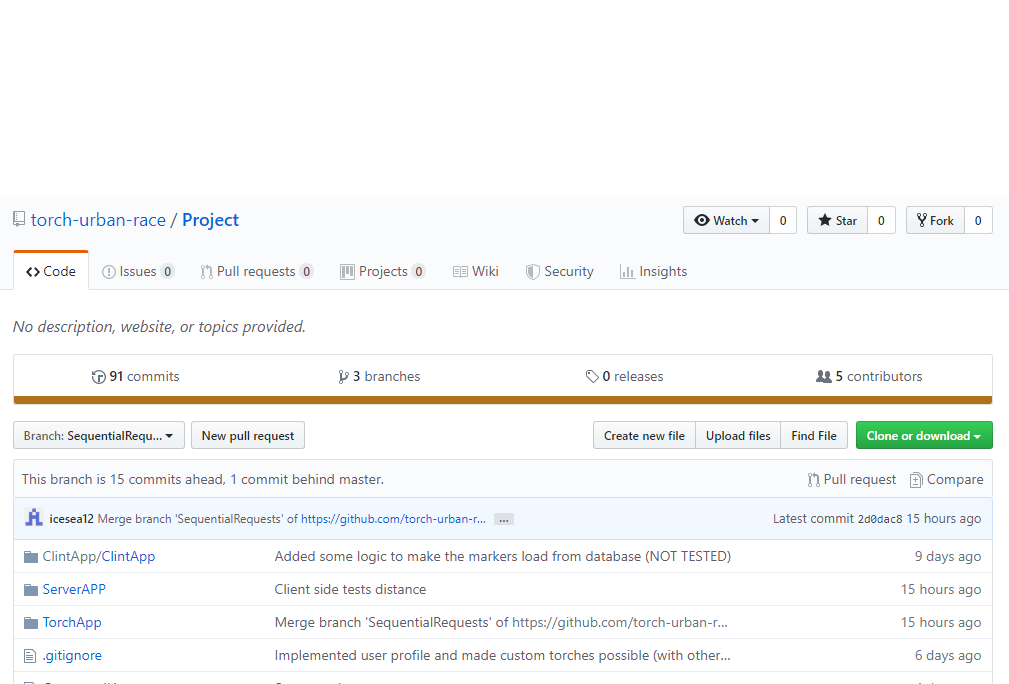
\includegraphics[width=1\linewidth]{GitHubProjectProgress.png}
     \captionsetup{justification=raggedright, singlelinecheck=false} 
     \caption{Screenshot of the GitHub repository.}
     \label{fig:GitHub}
 \end{figure}

 \newpage
 
 \begin{figure}
     \centering
     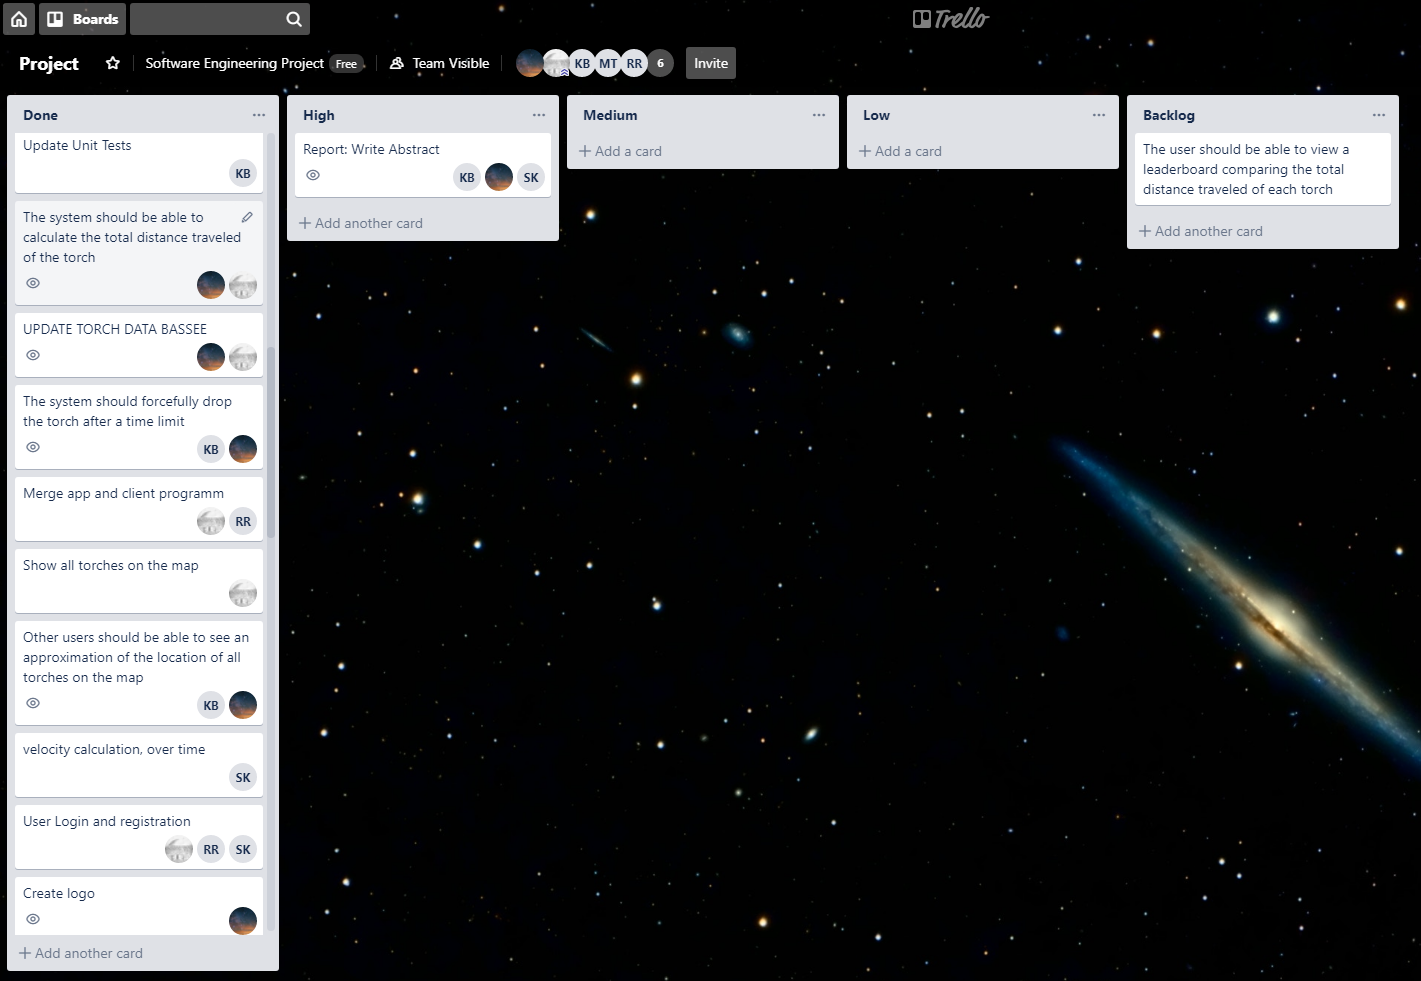
\includegraphics[width=1\linewidth]{TrelloProjectProgress.png}
     \captionsetup{justification=raggedright, singlelinecheck=false} 
     \caption{Screenshot of the Trello board.}
     \label{fig:Trello}
 \end{figure}
 
 \clearpage
%heeelllooooo

%hello!


\section{Results}

\subsection{Early development}

In the early stage after the group decided on the project and it was split. The priority of the project was to get the core features operational as soon as possible. Which for this project was getting the map and Google API operational and the sever up and running with access to the database. This would allow the team to later split up and create a more complete project.

\subsubsection{Google Api}
The first thing this project needed was an API key. It was essential to get access to that API in order to make use of its GPS features to track the users all-round the globe. Luckily, even though Google charges per request of their GPS system they offer a \$200 worth of service in free credit. This was more the enough for the whole entire development of the project. Using the Google services, we began constructing a map activity. Then, by using the Fused Location Provider - which uses the GPS, radio tower and WiFi, an accurate position of the player was obtained. This is an essential feature for a game based on GPS.


\subsubsection{Building the Map Activity}
 
 Now that user is being tracked correctly. The main feature of the game is to pickup torches scattered around the world. Taking advantage of the already built in markers feature in Google Maps API, only customizations were needed. The team made their own text and icons for the symbol of the torch.The basic UI elements were developed for interacting with the torches. In addition, using Google Maps API distance calculation formulas one could easily check the distance of the player position to the torch. This allowed limitations on how far away one has to be big to pick up a torch. to be set. Furthermore, a circle was added around the player's location to give a visual cue that the if the player is close enough to pick up the torch. 
 
 \begin{figure}
     \centering
     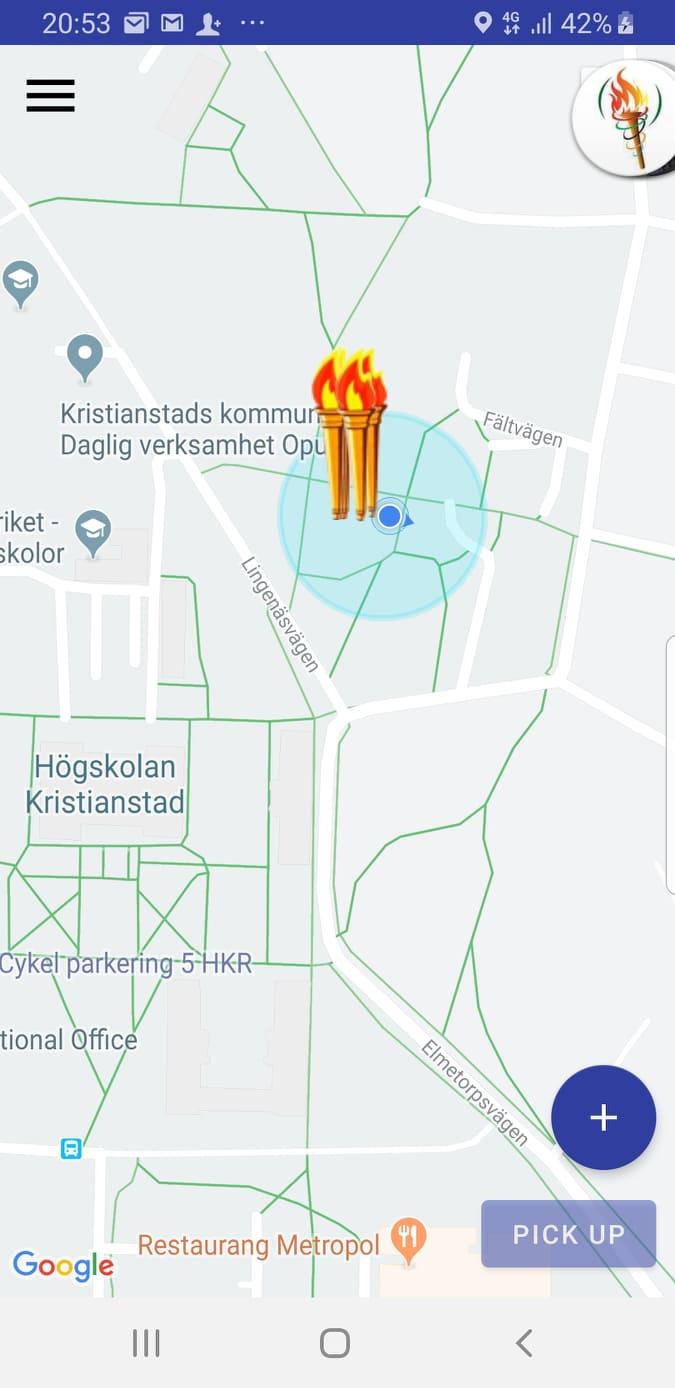
\includegraphics[width=0.3\linewidth]{torchPic.jpg}
     \caption{Screenshot of the app in the main map activity screen}
     \label{fig:my_label}
 \end{figure}
 \newpage
 
 
 \subsection{Client Sever Integration}
In order for the product to function as intended, a dedicated server was developed. The server acted as the gateway to a SQL database and had some utilities that allowed it to process data on behalf of the client. Such utilities included distance calculation and achievement awarding mechanisms. To integrate the two systems together the server functionality was developed first and then the client expanded to support the newly supported server requests. Each request was handled on a separate thread with the focus being to avoid any asynchronous queries on the main thread. Failing in doing so leads to application freezing, jitter or in worst case crashing.
 
 \subsection{Completing the Product}
With the core features completed and the database connected with the server. Work was done to round out the app for release. This includes a login / registration page, profile with stats tracker and a achievement page. Work was also done on the UI to make more friendly and intuitive to use for the players. 

\subsubsection{Achievements and Profile}
Icons were made for the achievements including one for the achievement that has yet to be completed. The user data with the achievement descriptions and rewards are fetched from the sever. Then, constructed into a customized achievements layout with the icons and dates on the client. Using a boolean the proper icon is displayed to show if the achievement has been completed. The stats are tracked by the database using the server and when the requirements are met the sever and database gets updated to award the achievement to the player. The rewards are applied subsequently.

 \begin{figure}
     \centering
     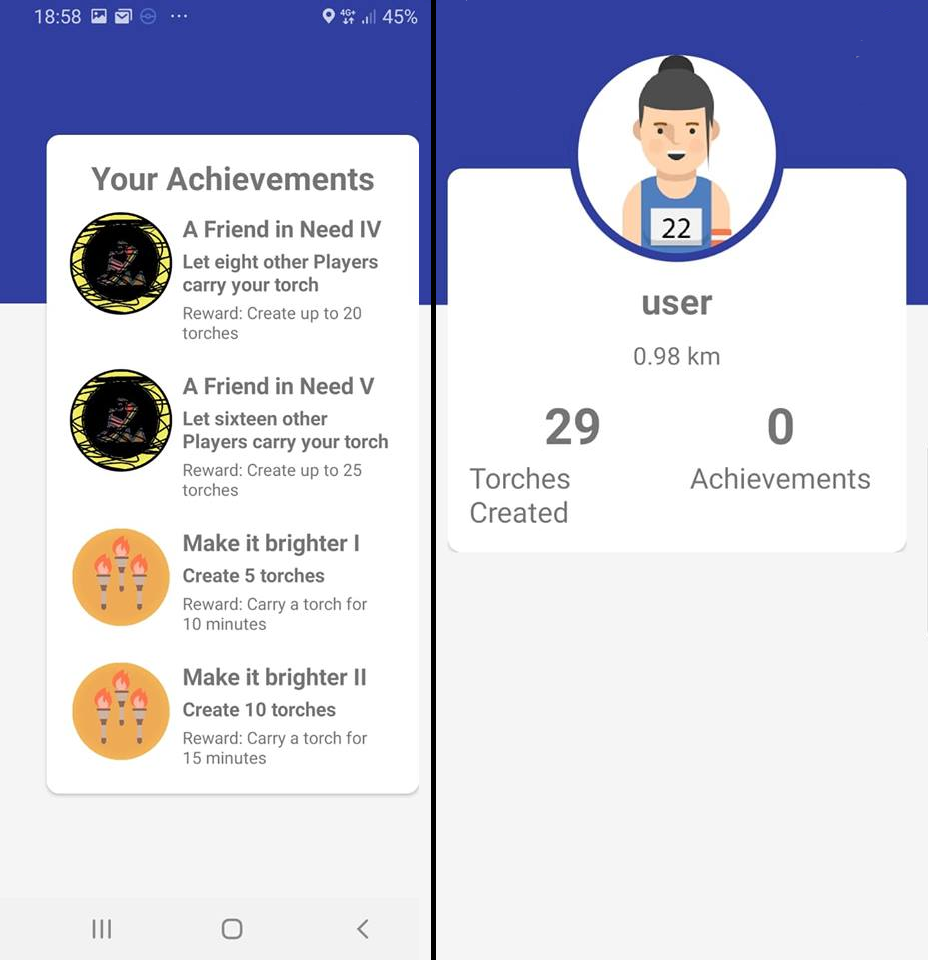
\includegraphics[width=0.5\linewidth]{achandprofiler.png}
     \caption{Screenshot of the app Achievements (left) and Profile page (right)}
     \label{fig:my_label}
 \end{figure}
 
 \subsection{Testing the Research Question}
 With the product ready the final stage was to create two versions of it. One version had processing distance on the client side, while the other on the server side. The two versions were tested under several conditions. The first condition was with varying torch numbers to put the system under stress, where the torches in the system went from a low number (3) to a high number (60). The second condition was about network stability, where the client was connected via 4G or Wi-Fi. The third condition was to test multi-threading performance where the server had to jump between clients. The final condition was tested between a single client up to 3. 

\subsubsection{The Number of Torches}

During the testing, the number of torches were increased from 3 torches to 60 torches, Using the system to track the response time form picking up of the torches. Increasing the number of torches increased the response time as you can see \autoref{Torchvstime} that there is upward trend in time. This is due to the fact that the increase of the torch in the system causes an increase in data that needs processing. This in turn affects the sever response time as the sever has to deal with the increase load from the data in the system. 


 \begin{figure}
     \centering
     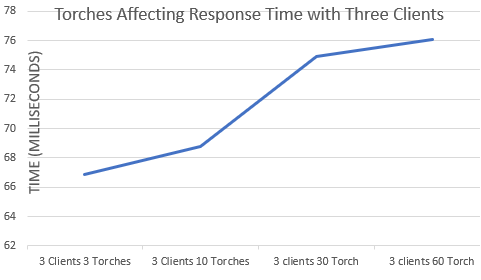
\includegraphics[width=0.5\linewidth]{Torchvstime.png}
     \caption{Data collected keeping the number of clients the same but increasing the number of torches. Notice the increasing in response time as the number of torches increases.}
     \label{Torchvstime}
 \end{figure}
 
 \newpage

\subsubsection{The Number of Clients}
Much like testing the number of torches, the number of clients was also increased from 1 to 3. Which as you can see in \autoref{TvsC} resulted in an increase in response time. Much like increasing the number of torches, increasing the number of clients also added extra stress to the sever. This test pushed the multi-threading capabilities of the system. While the difference is very small between one to three clients. This would have a very large effect if it was scaled to 10,000 clients, assuming the trend is maintained.

\begin{figure}
     \centering
     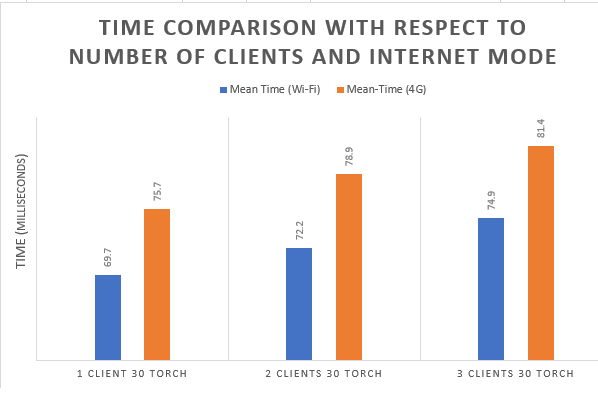
\includegraphics[width=0.5\linewidth]{TImecomparison.png}
     \caption{Data gather from when there was 30 torches on the map}
     \label{TvsC}
 \end{figure}
 

 \subsubsection{Using Wifi vs 4G}
 The difference between Wi-Fi and 4G seems indicate a loss of performance as well. This is partially due to the instability of the connection. The reason to suspect that is when calculating the standard deviation of the time measurements. 4G always stood out with a higher standard deviation which reached up to 98.
 
 
 \subsubsection{Client Side vs Sever Side }
 The epic conclusion to this investigation, When sever functions was moved client side the repose time decreased massively. The response time did not increase at all with the change of torches or client. This is because there is now a local reference to the torches in the system. This means the overhead to contact the server and for the server to access the database is mitigated. This allows the client to access the information rapidly and the subsequent mathematical calculations are easy to process by modern CPUs. The main bottleneck with such an approach is that older systems with less resources and computational power, might struggle to perform any complex operations. This could affect customers on the lower end of the performance spectrum from enjoying the services provided by the system.
 
 
 
 
  
 \begin{figure}
     \centering
     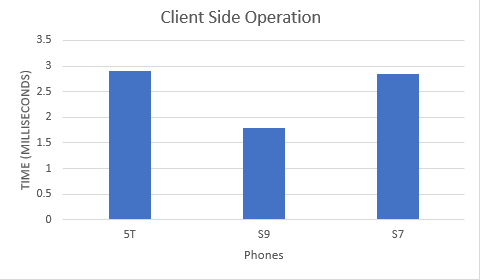
\includegraphics[width=0.5\linewidth]{CLIENTSIDEOP.png}
     \caption{Data gather from different brand phones, despite in changes in environment the only thing that affect the results was the performance of the phone.}
     \label{30torches}
 \end{figure}
 
\newpage
\section{Social and Ethical Aspects}
The social aspects that need to be considered are user privacy and security. Many people got hurt or even died in initial launches of Pokémon Go due to carelessness. Some people got robbed when going into remote areas to reach a Poké Stop or Arena which was set up for this purpose\cite{17}. This will need to be considered and prevented to the best of our abilities.There will also be a big possibility for advertisement. Using this responsibly will be crucial.

It important to make sure that we are not collecting any sensitive data that would be consider private data. Also to make sure that other user cant use the app to track other user and steal private information. Taking into account this it was changed in system to so the torches disappear when they are picked up. This means that you can't track the user. This will help in more dangerous countries to not get robbed as well.

Group environment was pleasant with people discussing ideas with each other or asking for help. Working as a team was a great experience for communication and collaborative skills. 

\newpage
\section{Discussion}

Despite the numerous limitations and lack of experience the team had coming into this project, the results were satisfying. It was a massive undertaking as none of the team members had experience working with android or the Google maps API. Neither experience when it comes to multiplayer client-server architecture. However, everything promised was delivered with only some minor aspects being delayed. When it comes to answering the research questions, the limitations were specified and the results obtained are in-line with what the literature study had stated. A more thorough and detailed analysis should be done if the results are to be added to the list of literature on the topic. However, the scope of this project and lack of resources has been a huge constraint to the findings.

Most of the challenges faced were lack in experience and knowledge, the only solution to that was spending extra time researching the topic and compensating through sharing. This means that if one team member has figured out something they can inform the rest of the team about it to save time.

\newpage
\section{Conclusion}

By the standards the team has set, the research question has been answered and the advantage / disadvantage stated. However, as by our long list of limitations the conclusion made might not fully represent the reality of the situation. Further research has been suggested in order to improve the results.

Overall, this project has been a very difficult learning experience. The team's inexperience with the technology combined with the scale necessary to test such systems posed as quite the challenge. However, using extreme programming and other methods this effort was rendered more manageable.

The team is proud of this system and are hoping to further enhance it to create a fun and engaging experience for its users.





\newpage
\section{Suggestions for Further Work}
Based on what was mentioned in limitations and discussion the following can be done to expand on this research. Testing client-side performance on similar devices to offset random variables in hardware differences. Testing on an actual industry grade server that was built with the intention of handling a lot of clients rather than a regular home PC. Testing different hardware systems to get a better insight into general performance metrics across different devices. Stress testing the system for stability using thousands of clients as performance is not the only metric that should matter (It was the focus of this research).

\newpage
\begin{thebibliography}{widestlabel}\addcontentsline{toc}{section}{\qquad Reference}

\bibitem{1}Barrett, B. (2018). THE QUIET, STEADY DOMINANCE OF POKÉMON GO. [online] wired. Available at: \url{http://www.chalmers.se/en/news} , cited Dec 12th 2017.

\bibitem{2}Barrett, B. (2018). THE QUIET, STEADY DOMINANCE OF POKÉMON GO. [online] wired. Available at: https://www.wired.com/story/pokemon-go-quiet-steady-dominance/ [28-04-2019].

\bibitem{3}Foreman, R. (2016). 4 Reasons Behind Pokémon Go’s Wild Success. [online] startupgrind. Available at: \url{https://www.startupgrind.com/blog/4-reasons-behind-pokemon-gos-wild-success/} [28-04-2019

\bibitem{4}Google Play (2019). Pokémon Go. [online] Available at: \url{https://play.google.com/store/apps/details?id=com.nianticlabs.pokemongo&gl=SE} [02-05-2019].

\bibitem{5}GPS.gov (2017). GPS Accuracy. [online] Available at: \url{https://www.gps.gov/systems/gps/performance/accuracy/} [28-04-2019].

\bibitem{6}Kastrenakes, J. (2017). GPS will be accurate within one foot in some phones next year. [online] THE VERGE. Available at: \url{https://www.theverge.com/circuitbreaker/2017/9/25/16362296/gps-accuracy-improving-one-foot-broadcom} [28-04-2019].

\bibitem{7}Rizzotto, L. (2018). The Real Reason Behind Pokemon Go’s Success. [online] Lucas Rizzotto’s Blog. Available at: \url{https://medium.com/futurepi/the-real-reason-behind-pokemon-gos-success-f938612bcd0d} [28-04-2019].

\bibitem{8}Van Diggelen, F., Want, R., Wei, W. (2018). How to achieve 1-meter accuracy in Android. [online] GPS WORLD. Available at: \url{https://www.gpsworld.com/how-to-achieve-1-meter-accuracy-in-android/} [28-04-2019].

\bibitem{9}Warman, P. (2016). Analysis of Pokémon GO: A Success Two Decades in the Making. [online] newzoo. Available at: \url{https://newzoo.com/insights/articles/analysis-pokemon-go/} [28-04-2019].

\bibitem{10}West, H. (2017). How Walking Can Help You Lose Weight and Belly Fat. [online] Healthline. Available at: \url{https://www.healthline.com/nutrition/walking-for-weight-loss} [Accessed 29 Apr. 2019].

\bibitem{11}Sharwood, S. (2019). Pokémon GO caused hundreds of deaths, increased crashes. [online] Theregister.co.uk. \url{https://www.theregister.co.uk/2017/11/27/pokemon_go_caused_car_accidents_and_deaths/ [Accessed 29 Apr. 2019]} .

\bibitem{12}Wikipedia (2019). Client-server model. [online] Available at: \url{https://en.wikipedia.org/wiki/Client%E2%80%93server_model} [02-05-2019].

\bibitem{13}Delahunty-Light, Z. (2019). Niantic was “caught off guard” by Pokemon Go’s early success, and admits the first Pokemon Go Fest could have gone better. [online] gamesradar. Available at: \url{https://www.gamesradar.com/niantic-was-caught-off-guard-by-pokemon-gos-early-success-and-admits-the-first-pokemon-go-fest-could-have-gone-better/} [Accessed 02-05-2019].

\bibitem{14}Silveira, R. (2019). Getting Started with Multiplayer Game Programming | Packt Hub. [online] Packt Hub. Available at: \url{https://hub.packtpub.com/getting-started-multiplayer-game-programming/} [Accessed 02-05-2019].

\bibitem{15}Luttu, J., and Rosquist, O. (2017). Analysis of the performance difference between server-side and client-side rendering for data visualization in real-time using d3.js. [pdf] Stockholm: KTH. Available at:  \url{http://www.diva-portal.org/smash/get/diva2:1107724/FULLTEXT01.pdf} [Accessed 02-05-2019].

\bibitem{16}Xian, Y., 2017. An Initial Evaluation of the Impact of Pokémon GO on Physical Activity. [Online] Available at: \url{https://www.ahajournals.org/doi/10.1161/JAHA.116.005341} [Accessed 15 April 2019].

\bibitem{17}Dax, H., 2017. What are the disadvantages of Pokémon GO?. [Online] Available at: \url {https://www.quora.com/What-are-the-disadvantages-of-Pokémon-GO}[Accessed 17 April 2019].

\bibitem{18}Eilertsen, V. (2017). The Olympic torch relay: “a symbol of peace, friendship, tolerance and hope”. [online] International Olympic Committee. Available at: \url{https://www.olympic.org/news/the-olympic-torch-relay-a-symbol-of-peace-friendship-tolerance-and-hope}. [Accessed 26 Apr. 2019].


\newpage
\section{Appendix}

\subsection{Charts}

 \begin{figure}[htps]
     \centering
     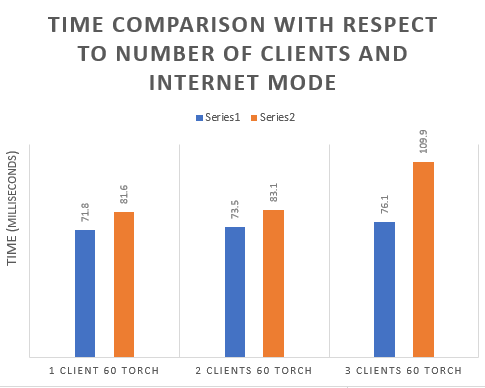
\includegraphics[width=0.5\linewidth]{tc1.png}
     \caption{For the test done with 60 torches on the map}
     \label{60torch}
 \end{figure}
 
 
 \begin{figure}[htps]
     \centering
     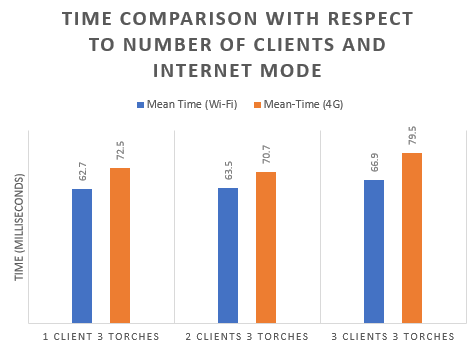
\includegraphics[width=0.5\linewidth]{tc2.png}
     \caption{For the test done with 3 torches on the map)}
     \label{3torch}
 \end{figure}
 
  \begin{figure}[htps]
     \centering
     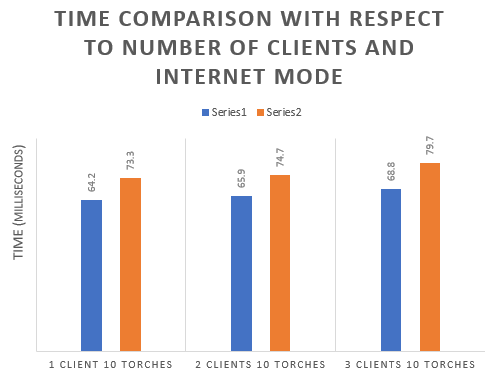
\includegraphics[width=0.5\linewidth]{tc3.png}
     \caption{For the test done with 10 torches on the map}
     \label{10torch}
 \end{figure}
 
 \subsection{Screen Shots of phone}
  \begin{figure}[htps]
     \centering
     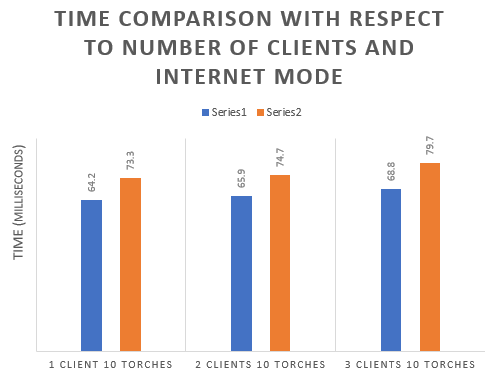
\includegraphics[width=0.5\linewidth]{tc3.png}
     \caption{For the test done with 10 torches on the map}
     \label{10torch}
 \end{figure}


\end{thebibliography}



%\begin{figure}[htp!]
%\centering
 %\includegraphics[width=0.9\linewidth]{TEK00001.PNG}
  %\captionsetup{justification=raggedright, singlelinecheck=false} 
%\caption{Screenshot of the oscilloscope measuring a sinus potential with a Vpp of 2V and frequency of 1kHz..}
%\label{1}  
%\end{figure}

















\end{document}